% Set up by Kristyna Kantnerova on 18-May-2022
% https://orcid.org/0000-0001-6259-3225
% https://github.com/SabrielxD

\documentclass[a4paper,12pt]{article}

\usepackage{master_thesis_style} % loading the style package

% a path to figures
\graphicspath{{figures/}}

%% BEGINNING OF THE DOCUMENT
\begin{document}

\pagestyle{empty}

%% Abstract
% cesky
\large
\noindent
\textbf{SOUHRN}

\vspace{5mm}
\noindent
\normalsize
\textbf{Název práce}

\vspace{5mm}

\begingroup
\fontsize{12}{11.5}\selectfont
\noindent

% text abstraktu
\lipsum[1-3]

\endgroup

\newpage
% English
\large
\noindent
\textbf{SUMMARY}

\vspace{5mm}
\noindent
\normalsize
\textbf{Thesis title}

\vspace{5mm}

\begingroup
\fontsize{12}{11}\selectfont
\noindent

% abstract text
\lipsum[1-3]

\endgroup





%% Acknowledgement
\newpage
\section*{ACKNOWLEDGEMENT}
% acknowledgement
\lipsum[1-3]


\newpage
\tableofcontents

%% Main part
\newpage
\pagestyle{plain}
\section{INTRODUCTION}
% introduction

\lipsum[1]
\\

\textbf{This is an example of an inserted png figure with a reference label -- Fig.~\ref{fig:opaipatpa}.}
 
\begin{figure}[!ht]
  \centering
 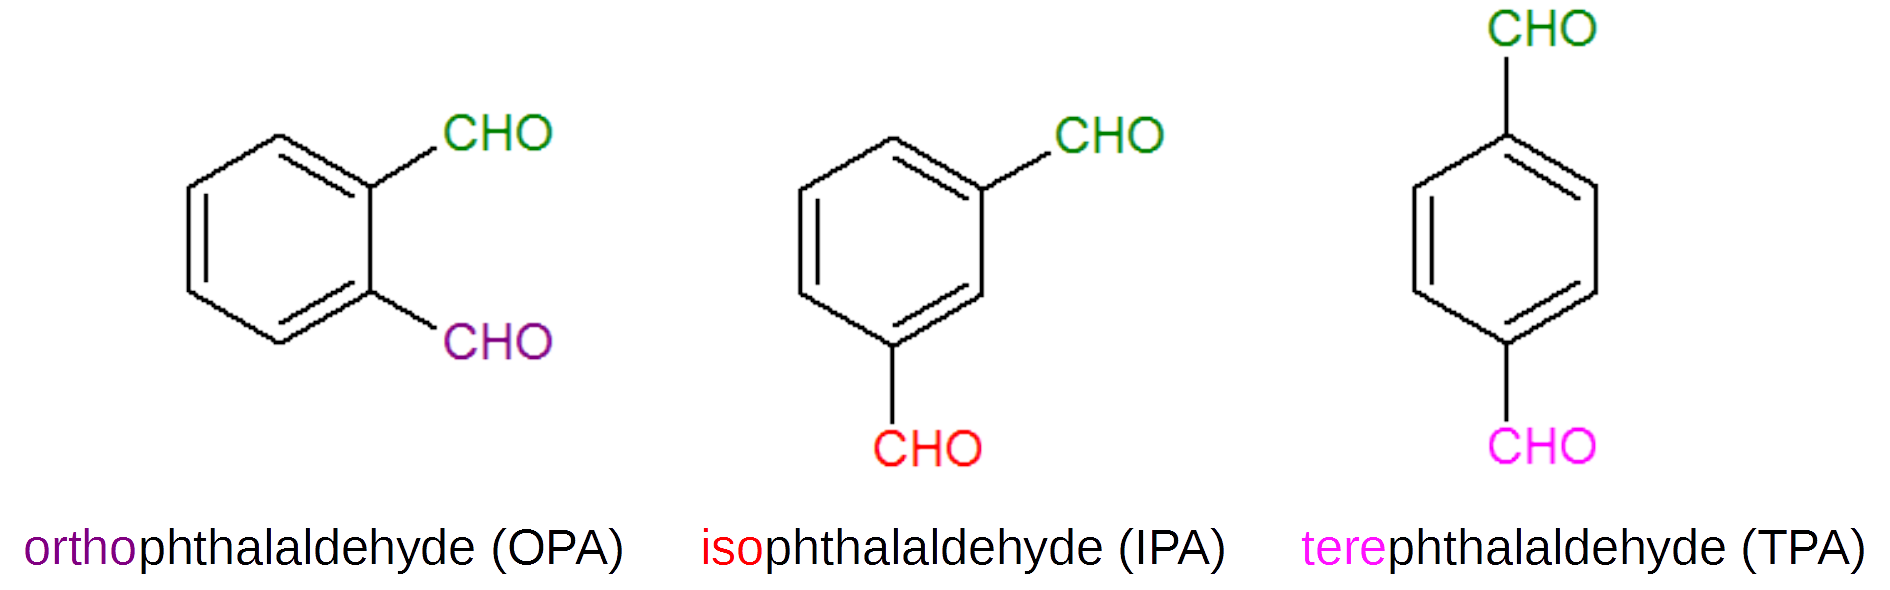
\includegraphics[width=13cm]{opaipatpa.png}
 \caption{Structures of OPA, IPA and TPA.}
 \label{fig:opaipatpa}
\end{figure}

\textbf{This is an example of literature reference.}\cite{McKenzie2002} \\

\label{chap:Introduction}
\clearpage

\newpage
\section{LITERATURE}
\subsection{Subsection 1}
\label{sec:subsection1}
\textbf{This is an example of a double reference.}\cite{Peace2005,Dai2014} 

\subsection{Subsection 2}
\label{sec:subsection2}

As was mentioned in \textbf{the previous subsection \ref{sec:subsection1}}, ...

\subsubsection{Subsubsection 2.1}
\label{sec:subsubsec2.1}

Ninhydrin (structure in \textbf{Fig.~\ref{fig:ninhydrin}}) ...

\begin{figure}[!ht]
  \centering
 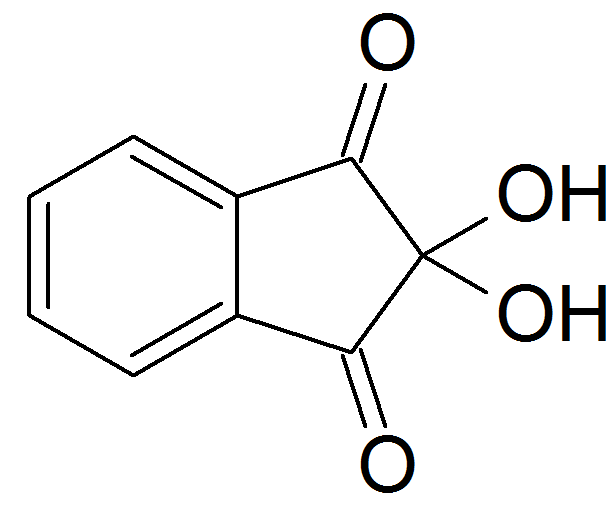
\includegraphics[width=3cm]{ninhydrin.png}
 \caption{Structure of ninhydrin.}
 \label{fig:ninhydrin}
\end{figure}
\label{chap:Literary part}
\clearpage

\newpage
\section{EXPERIMENT}
% experimental part
\subsection{Subsection 1}
\label{sec:subsection_exp_1}

\textbf{Below are few examples of using the siunitx package.}\\

The DME is a capillary tube with inner diameter approx.~\SI{50}{\micro\meter}, which is connected with the mercury reservoir. The drop time was \SI{1}{\second}, scan rate was \SI{10}{\mV/\second}. Cyclic voltammetry (CV) is a linear scan voltammetry that is characteristic with faster scan rate (from \SI{50}{\mV/\second} to \SI{100}{\mV/\second} for standard analytical working electrodes with the size about 1 mm$^2$), which makes the experiment time-dependent.\cite{Bard}  

For measuring CV before and after electrolysis, a mercury "pseudodrop" electrode was used. It consists of a platinum wire which has a small sphere at one end with diameter approx. \SI{1}{\milli\meter}. The rest of the wire is sealed into a glass tube and used as a contact. The small sphere is immersed into a saturated solution of AgNO$_3$ together with a counter electrode. Electrolysis is performed at potential \SI{-1}{\volt} for \SI{5}{\minute} and by that the sphere is covered with silver. After that the electrode is immersed into mercury and silver amalgam is formed at the surface of the sphere. For renovation of the mercury surface, the tip of the electrode is again immersed into mercury. After several tens of measurements, the sphere has to be renewed. For that, electrolysis is performed in a 10\% solution of HNO$_3$ at potential \SI{1}{\volt}; by that, the silver sphere dissolves and it can be created again.

\subsection{Subsection 2}
\label{sec:subsection_exp_2}

Equation~\ref{eq:einstein} serves as \textbf{an example of a mathematical equation}.

\begin{equation}
E = mc^2
\label{eq:einstein}
\end{equation}

\noindent
It can be written also directly inline as \(E=mc^2\).
\label{chap:Experimental part}
\clearpage

\newpage
\section{RESULTS AND DISCUSSION}
\lipsum[1]

\subsection{Subsection 1}
\label{sec:subsection_res_1}

\lipsum[2]

\subsubsection{Subsubsection 1.1}
\label{sec:subsubsec_res_1.1}

\lipsum[3]

\subsubsection{Subsubsection 1.2}
\label{sec:subsubsec_res_1.2}

\lipsum[4]

% example of a plot with referring to it

Based on the possible structure of the product and on other obtained information, a probable reduction mechanism can be drawn (Fig.~\ref{fig:IR_OPAmech}). 

\begin{figure}[!ht]
  \centering
 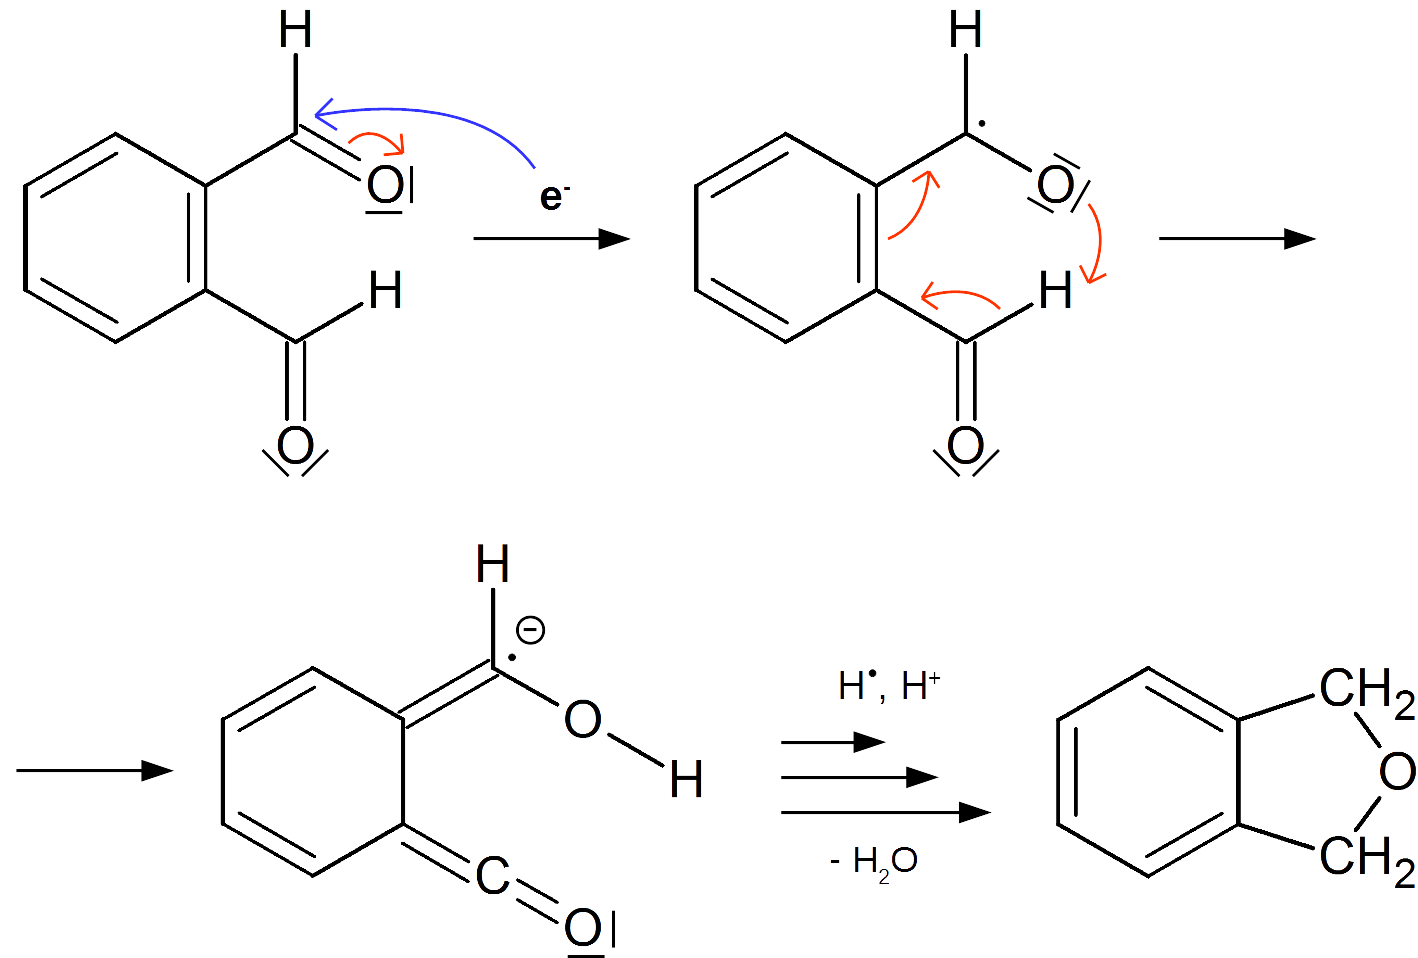
\includegraphics[width=11cm]{IR_OPAmech.png}
 \caption{A proposed mechanism for the first step of the OPA reduction.}
 \label{fig:IR_OPAmech}
\end{figure}

% following is an example of a broader plot on an individual landscape page

\begin{landscape}
\begin{figure}[!ht]
  \centering
 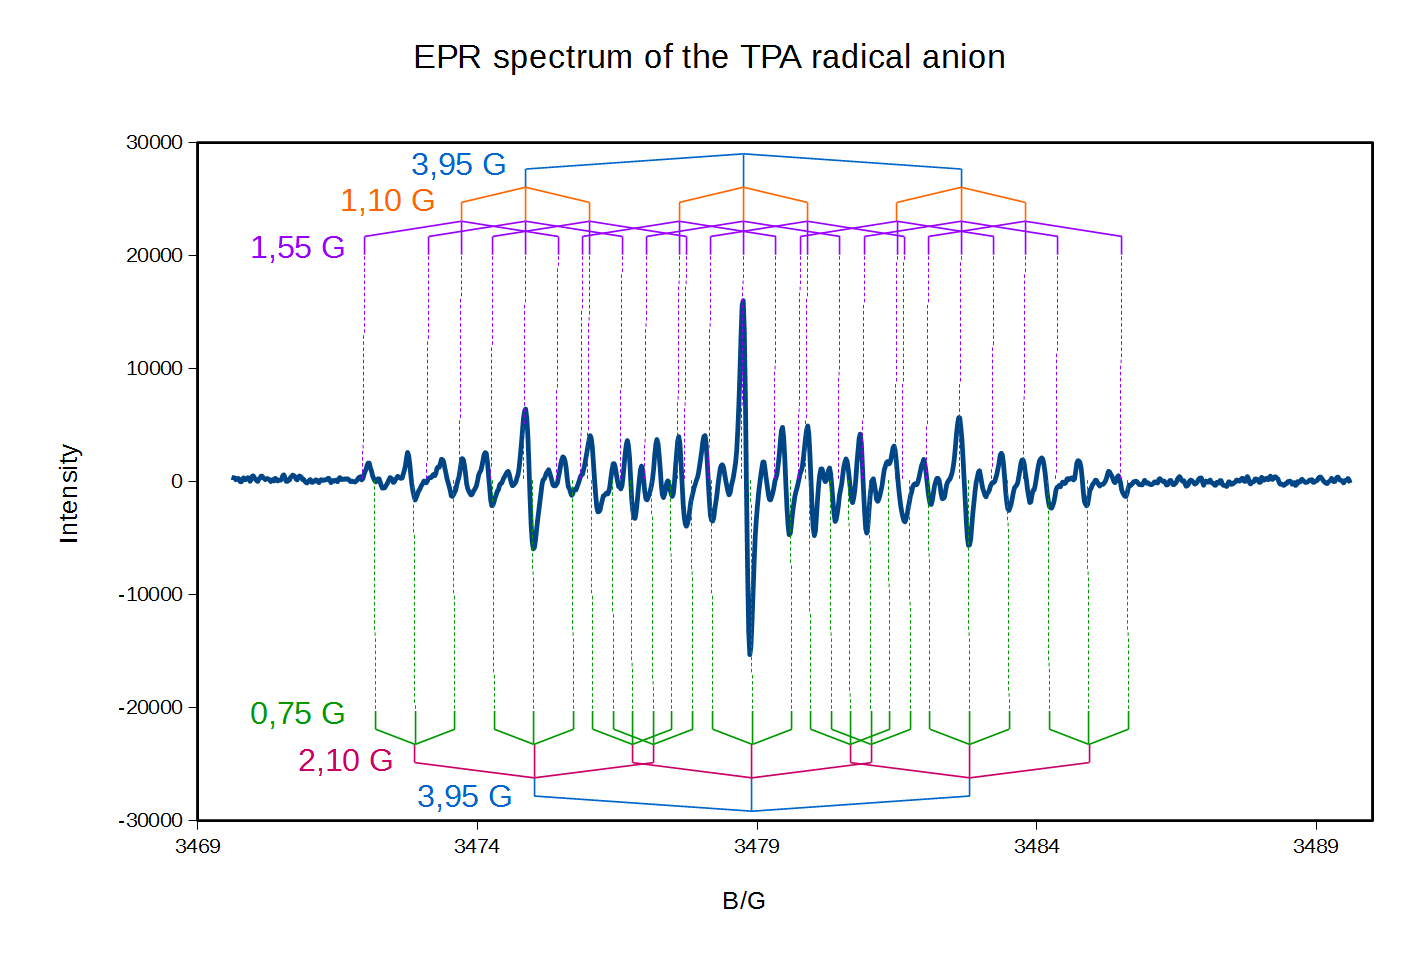
\includegraphics[width=18cm]{EPR_TPA.png}
 \caption[EPR spectrum of the TPA radical anion.]{EPR spectrum of the TPA radical anion generated electrochemically \textit{in~situ} in the EPR cavity. Derived coupling constants for the \textit{cis} and \textit{trans} rotamer are displayed above and below the spectrum.}
 \label{fig:EPR_TPA}
\end{figure}

\end{landscape}

% example of a table with a reference

Table~\ref{tab:tableXPABA} summarizes reduction potentials and the electron consumptions in both steps. For comparison of the reduction behavior, the value of reduction potential of benzaldehyde is given.

\begin{table}[htb]
\centering
\caption{Reduction potentials and the electron consumptions for studied benzenedialdehydes in ACN and comparison with benzaldehyde (BA).}
\begin{tabular}{ c c c c c c }
\toprule
& $E_{red}^1$/V & $z_1$ & $E_{red}^2$/V & $z_2$ & $E_{red}^3$/V  \\ 
\midrule
    OPA & $-1.51$ & 0.40 & $-2.02$ & 1 & ($-2.20$) \\ 
	IPA & $-1.68$ & 0.80 & $-2.04$ & $>$ 1 & -- \\ 
	TPA & $-1.46$ & 0.35 & $-1.90$ & $<$ 1 & -- \\ 
	BA\cite{Mairanovskii1976} & \ & \  & $-2.00$  & \ &  \\ 
\bottomrule
\end{tabular}
\label{tab:tableXPABA}
\end{table}

% example of a more complex table with a multicolumn

\begin{table}[!ht]
  \begin{center}
	\caption{Reduction potentials from CV for OPA in ACN, DMF and acetone and on mercury and gold electrode. Potentials are related to the SCE.}
  \label{tab:OPAnevoda}
  \footnotesize
	\renewcommand{\arraystretch}{1.4}
\begin{tabular}{ >{\centering\arraybackslash} m{1.7cm}  c  c  c  c  c  c  c  }
\toprule
	\shortstack{solvent/\\electrode} & E$_{pc}^1$/V & E$_{pa}^1$/V & $\Delta$E$^1$/mV & E$_{pc}^2$/V & E$_{pa}^2$/V & $\Delta$E$^2$/mV & E$_{pc}^3$/V \\  
\midrule[0.3mm]	
	  ACN/Hg & $-1.51$  & $-1.45$ & 60 & $-2.02$ & -- & -- & $-2.20$   \\ 
	  DMF/Hg & $-1.41$ & $-1.35$ & 60 & $-2.10$ & $-2.02$ & 80 & --   \\ 
	  DMF/Au & $-1.44$ & $-1.37$ & 70 & -- & -- & -- & --   \\ 
	  acetone/Hg & \multicolumn{7}{c}{the substance probably reacts with the solvent} \\ 
\bottomrule	   
\end{tabular}
\end{center}
\end{table}

% another table example

\begin{table}[!ht]
  \begin{center}
	\caption{Slopes from \emph{ln(i)-t} curves for the ratio AA:OPA 3:1}
  \label{tab:slopesAAs}
	\renewcommand{\arraystretch}{1.4}
\begin{tabular}{l >{\centering\arraybackslash}m{2.5cm} >{\centering\arraybackslash}m{2.5cm}}
\toprule
\multicolumn{1}{c}{AA:OPA 3:1}  & \multicolumn{2}{c}{slope: $\frac{dln(i)}{dt}\cdot10^3$} \\ 
 \toprule
\multicolumn{1}{c}{amino acid}  & pH 7.86    & pH 11.22 \\ 
\midrule[0.3mm]
   glycine                         & -3.20   & -3.65  \\
   alanine                         & -2.00   & -5.10 \\ 
	 $\alpha$-aminobutyric acid      & -1.70   & -4.70 \\
	 $\alpha$-aminoisobutyric acid   & -0.04   & -0.20 \\
	 valine                          & -1.40   & -2.70 \\
	 norvaline                       & -1.70   & -4.25 \\
	 leucine                         & -1.75   & -3.80 \\
	 isoleucine                      & -1.40   & -2.90 \\
\bottomrule
\end{tabular}
\end{center}
\end{table}

\label{chap:Results}
\clearpage

\newpage
\section{CONCLUSION}
% conclusion
\lipsum[1-3]


\label{chap:Conclusion}
\clearpage

\newpage
\section*{LIST OF ABBREVIATIONS}
\addcontentsline{toc}{section}{List of abbreviations}

\textbf{Two examples of lists -- manual and automatic alphabetic sorting:}

% example - manual alphabetic sorting

\begin{longtable}{ p{.15\textwidth}  p{.75\textwidth} }

IPA & isophthalaldehyde\\

OPA & orthophthalaldehyde\\

TPA & terephthalaldehyde\\

\end{longtable}

% example - automatic alphabetic sorting

\begin{sortedlist}
    \sortitem{QCLAS -- quantum cascade laser absorption spectroscopy}
    \sortitem{TREX -- TRace gas EXtractor}
    \sortitem{IR -- infrared}
    \sortitem{QCL -- quantum cascade laser}
\end{sortedlist}

%% List of figures 
\clearpage
\listoffigures

%% List of tables
\clearpage
\listoftables

%% Supplementary materials
\newpage
\section*{SUPPLEMENTARY MATERIAL}
% adding it to the table of contents
\addcontentsline{toc}{section}{SUPPLEMENTARY MATERIAL}
\appendix

% A - Supplementary tables
\section{\fontsize{12}{12}\selectfont Tables}
\label{AppendixA}
\input{chapters/supplementary_tables.tex}
\clearpage

% B - Supplementary plots
\section{\fontsize{12}{12}\selectfont Plots}
\label{AppendixB}
\input{chapters/supplementary_plots.tex}
\clearpage

%%% List of references
\bibliography{papers} % if you have multiple bib files, never put space after comma

\end{document}
